\documentclass[journal]{IEEEtran}
\usepackage{graphicx}
\usepackage[outdir=./]{epstopdf}
\usepackage{subfigure}
\usepackage{hyperref}
\usepackage{booktabs}
\usepackage[table]{xcolor}
\usepackage{multirow}
\usepackage{cleveref}
\usepackage[utf8]{inputenc}
\usepackage[spanish, mexico]{babel}
\usepackage{amsmath}
\usepackage{algorithm}
\usepackage{algorithmic}
\floatname{algorithm}{Algoritmo}
\renewcommand{\listalgorithmname}{Lista de algoritmos}
\renewcommand{\algorithmicrequire}{\textbf{Entrada:}}
\renewcommand{\algorithmicensure}{\textbf{Salida:}}
\renewcommand{\algorithmicend}{\textbf{fin}}
\renewcommand{\algorithmicif}{\textbf{si}}
\renewcommand{\algorithmicthen}{\textbf{entonces}}
\renewcommand{\algorithmicelse}{\textbf{si no}}
\renewcommand{\algorithmicelsif}{\algorithmicelse,\ \algorithmicif}
\renewcommand{\algorithmicendif}{\algorithmicend\ \algorithmicif}
\renewcommand{\algorithmicfor}{\textbf{para}}
\renewcommand{\algorithmicforall}{\textbf{para todo}}
\renewcommand{\algorithmicdo}{\textbf{hacer}}
\renewcommand{\algorithmicendfor}{\algorithmicend\ \algorithmicfor}
\renewcommand{\algorithmicwhile}{\textbf{mientras}}
\renewcommand{\algorithmicendwhile}{\algorithmicend\ \algorithmicwhile}
\renewcommand{\algorithmicloop}{\textbf{repetir}}
\renewcommand{\algorithmicendloop}{\algorithmicend\ \algorithmicloop}
\renewcommand{\algorithmicrepeat}{\textbf{repetir}}
\renewcommand{\algorithmicuntil}{\textbf{hasta que}}
\renewcommand{\algorithmicprint}{\textbf{imprimir}} 
\renewcommand{\algorithmicreturn}{\textbf{devolver}} 
\renewcommand{\algorithmictrue}{\textbf{cierto }} 
\renewcommand{\algorithmicfalse}{\textbf{falso }} 

\usepackage{color}
\usepackage{listings}
\lstset{ %
language=Matlab,                % choose the language of the code
basicstyle=\footnotesize,       % the size of the fonts that are used for the code
numbers=left,                   % where to put the line-numbers
numberstyle=\footnotesize,      % the size of the fonts that are used for the line-numbers
stepnumber=1,                   % the step between two line-numbers. If it is 1 each line will be numbered
numbersep=5pt,                  % how far the line-numbers are from the code
backgroundcolor=\color{white},  % choose the background color. You must add \usepackage{color}
showspaces=false,               % show spaces adding particular underscores
showstringspaces=false,         % underline spaces within strings
showtabs=false,                 % show tabs within strings adding particular underscores
frame=single,           % adds a frame around the code
tabsize=2,          % sets default tabsize to 2 spaces
captionpos=b,           % sets the caption-position to bottom
breaklines=true,        % sets automatic line breaking
breakatwhitespace=false,    % sets if automatic breaks should only happen at whitespace
escapeinside={\%*}{*)}          % if you want to add a comment within your code
}
%%%%%%%%%%%%%%%%%%%%%%%%%%%%%%%%%%%%%%%%%%%%%%%%%%%%%%%%%%%%%%%%%
%% The following definitions are to extend the LaTeX algorithmic 
%% package with SWITCH statements and one-line structures.
%% The extension is by 
%%   Prof. Farn Wang 
%%   Dept. of Electrical Engineering, 
%%   National Taiwan University. 
%% 
%\algnewcommand\algorithmicswitch{\textbf{switch}}
%\algnewcommand\algorithmiccase{\textbf{case}}
%\algnewcommand\algorithmicassert{\texttt{assert}}
%\algnewcommand\Assert[1]{\State \algorithmicassert(#1)}%
%\algdef{SE}[SWITCH]{Switch}{EndSwitch}[1]{\algorithmicswitch\ #1\ \algorithmicdo}{\algorithmicend\ \algorithmicswitch}%
%\algdef{SE}[CASE]{Case}{EndCase}[1]{\algorithmiccase\ #1}{\algorithmicend\ \algorithmiccase}%
%\algtext*{EndSwitch}%
%\algtext*{EndCase}%
%% 
%% End of the LaTeX algorithmic package extension.
%%%%%%%%%%%%%%%%%%%%%%%%%%%%%%%%%%%%%%%%%%%%%%%%%%%%%%%%%%%%%%%%%


%\usepackage{float}
\usepackage{mathpazo}
\begin{document}

% Corregir problemas de separación de palabras por guiones
%\hyphenation{op-tical net-works semi-conduc-tor}

\floatname{algorithm}{Pseudocódigo}
\title{Análisis lineal discriminante (\emph{LDA})}

\author{Rafael~Pérez~Torres \\
	Profesor: Dr. Wilfrido Gómez Flores,\\[6pt]\IEEEmembership{LTI Cinvestav}.
	
	%\thanks{Rafael Pérez Torres es estudiante de doctorado en Ciencias de la Computación en el Laboratorio de Tecnologías de Información del CINVESTAV, email: rperez@tamps.cinvestav.mx.}
}

\markboth{Reconocimiento de patrones, Abril~2015}%
{Pérez Torres: Reconocimiento de patrones}

\maketitle

\begin{abstract}
El análisis lineal discriminante (\emph{LDA}) es una técnica para la reducción de dimensionalidad que también puede ser utilizada para realizar clasificación lineal supervisada.
\emph{LDA} permite reducir la dimensionalidad de un conjunto de datos de $l$ dimensiones proyectándolos en $c-1$ dimensiones, donde $c$ es la cantidad de clases del conjunto de datos.
Los datos proyectados pueden entonces describir una separación lineal, la cual es utilizada para realizar la clasificación de los mismos.

En su forma general, \emph{LDA} permite realizar clasificación binaria, sin embargo esto es suficiente para realizar incluso la clasificación multiclase al seguir un enfoque como \emph{uno vs uno} o \emph{uno vs todos}.
El enfoque \emph{uno vs todos} busca realizar $c$ clasificaciones binarias en las que se obtiene el grado de pertenencia de la instancia a una clase en específico o al resto de ellas, asignando aquella clase en la que la pertenencia es mayor.

El presente documento describe la implementación de \emph{LDA} para clasificación multiclase, utilizando el enfoque de \emph{uno vs todos} sobre ocho datasets sintéticos, así como la presentación de los porcentajes de error obtenidos.
\end{abstract}

\begin{IEEEkeywords}
Reconocimiento de patrones, LDA
\end{IEEEkeywords}

\section{Introducción}
\label{sec:introduccion}
El análisis lineal discriminante, \emph{LDA}, es una generalización del discriminante lineal de Fisher, creada por el estadístico, biólogo y matemático Ronald Fisher.

\emph{LDA} es una técnica que puede ser empleada tanto para clasificación como para reducción de dimensionalidad de un conjunto de datos previo a la clasificación.
El objetivo básico del \emph{LDA} es la búsqueda de una combinación lineal de atributos que separen de la mejor forma a las clases.

Esta reducción de la dimensionalidad puede entenderse fácilmente observando la Figura \ref{fig:proyecciones}.
En ella se muestran dos ejemplos en el que se ha reducido la dimensionalidad de los datos, que obedecen a dos clases (roja y azul), a solamente una dimensión.
Los datos son proyectados entonces de su espacio original, logrando describir sus características en apenas una sola dimensión.
Sin embargo, tal como se muestra en la Subfigura \ref{fig:mal-lda}, no todas las proyecciones resultan ser convenientes para realizar esta reducción ya que no se logra reflejar una mejor separabilidad de los datos.
En cambio, la Subfigura \ref{fig:buen-lda} muestra un \emph{buen} ejemplo de proyección en el que, a pesar de tener solamente una dimensión, se hace posible separar fácilmente al conjunto de datos en las dos clases originales.
\begin{figure*} 
\centering 
	\subfigure[\emph{Mala} proyección]{\label{fig:mal-lda}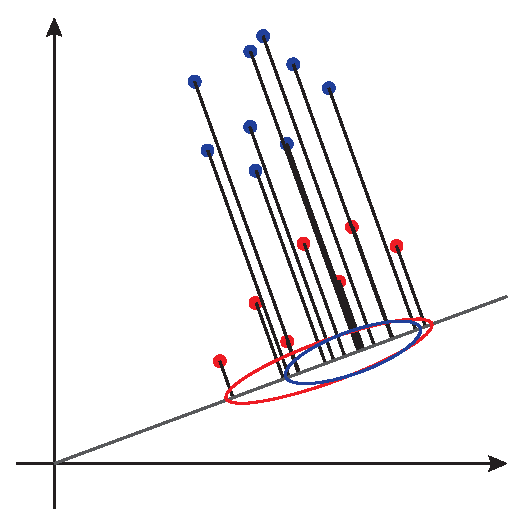
\includegraphics[scale=0.7]{imagenes/mal-lda}}
	\subfigure[\emph{Buena} proyección]{\label{fig:buen-lda}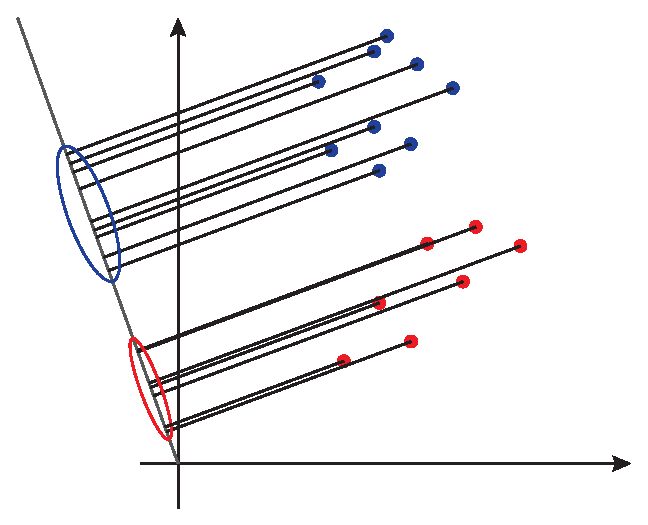
\includegraphics[scale=0.7]{imagenes/buen-lda}}

	\caption{Ejemplo de proyecciones}
	\label{fig:proyecciones}
\end{figure*}


Usando la misma Figura \ref{fig:proyecciones} es posible observar también que el \emph{LDA} utiliza como características clave la media y varianza de cada una de las clases, intentando maximizar la relación de las varianza interclase (datos de distintas clase) así como la relación intraclase (datos de la misma clase), de tal forma que las proyecciones obtenidas posicionen a los datos en grupos \emph{densos} y altamente separados.

Como dato adicional, es importante destacar que \emph{LDA} asume que las distribuciones de los datos son gaussianas, obteniendo resultados no satisfactorios si los datos carecen de dicha característica.

\section{Marco teórico}
A través de una función de regresión lineal, como $$f(x;w) = w^Tx$$ es posible proyectar cada punto $\mathbf{x} = [x_1,x_2,...,x_l]^T$ de un dataset hacia una línea paralela al vector de proyecciones $\mathbf{w}$ que pasa por el origen.

Entonces, variando este vector de proyecciones, o pesos si se hace la analogía con los clasificadores lineales abordados en clase, es posible obtener diferentes niveles de separación, tal y como se mostraba en las gráficas de la Figura \ref{fig:proyecciones}.
El objetivo del LDA es precisamente encontrar el vector de proyecciones $\mathbf{w^*}$ que maximice la separación entre las clases proyectadas.

De esta forma, la bondad de un vector de proyecciones viene definida por una medida de separación, como por ejemplo la diferencia entre la media de los datos de cada clase.
Sin embargo, la media no siempre obtiene valores óptimos de separación por lo que se involucra otra característica de los datos tal como la varianza.

El criterio de Fisher, base para \emph{LDA}, consiste precisamente en una función lineal $w^Tx$ que considera tanto a la media como a la varianza de los datos, intentando maximizar (para dos clases) a:
\begin{equation}
separacion= \frac{|( \mu_1 - \mu_2 ) |^2}{s_1^2 + s_2^2} \label{eq:criterio-fisher}
\end{equation}
%$$J(\mathbf{w})= \frac{|( \mu_1 - \mu_2 ) |^2}{\tilde{s}_1^2 + \tilde{s}_2^2}$$
%$$J(\mathbf{w})=\frac{\tilde{\mu}_1 - \tilde{\mu}_2}{\tilde{s}_1^2 + \tilde{s}_2^2} = \frac{|\mathbf{w}^T( \mu_1 - \mu_2 ) |^2}{\tilde{s}_1^2 + \tilde{s}_2^2}$$
donde $\mu_1$ y $\mu_2$ son los valores de las medias y $s_1^2$ y $s_2^2$ son los valores de las varianzas de las clases en la dimensión original.

Asumiendo que es posible encontrar el valor del vector de proyección $\mathbf{w}$, utilizar \emph{LDA} para clasificación involucraría realizar las etapas de entrenamiento y la clasificación como tal:
\begin{itemize}
	\item Entrenamiento: Las actividades se concentrarían en calcular el vector de proyección $\mathbf{w}$ y un bias.
	\item Clasificación. Las actividades se concentrarían en evaluar cada patrón desconocido con los vectores de proyección de cada clase y tomar aquel que arroje el valor más alto.
\end{itemize}

Las siguientes subsecciones describen el marco teórico de ambas tareas.

\subsection{Entrenamiento del LDA} % (fold)
\label{sub:entrenamiento_del_lda}

% subsection entrenamiento_del_lda (end)
Ahora bien, para expresar lo anterior en términos del vector de proyección $\mathbf{w}$ es preciso reiterar que basta con \emph{proyectar} cada punto en el nuevo espacio de dimensiones; esto se consigue multiplicando cada punto por este vector.
De esta manera, la distancia entre las medias proyectadas puede ser expresada a través de:
\begin{equation}
|\tilde{m}_1 - \tilde{m}_2| = |\mathbf{w}^T (\mu_1 - \mu_2)|
\end{equation}

Si se definen las matrices de dispersión $S_i$ y $S_w$ como:
\begin{equation}
S_i = \sum_{x\in\omega_i}(\mathbf{x}-\mu_i)(\mathbf{x} - \mu_i)^T
\end{equation}
y
\begin{equation}
S_w = S_1 + S_2
\end{equation}
Entonces la varianza de los datos proyectados de cada clase $\omega_i$ puede ser expresada en términos de matrices de dispersión, como en:

\begin{eqnarray}
\tilde{s}_i^2 &=& \sum_{x\in\omega_i}{(x-\tilde{\mu}_i)^2} \label{eq:varianzas} \\ 
&=& \sum_{x\in\omega_i}{(\mathbf{w}^Tx-\mathbf{w}^T\mu_i)^2} \\
&=& \sum_{x\in\omega_i}{\mathbf{w}^T(\mathbf{x}-\mu_i)(\mathbf{x} - \mu_i)^T\mathbf{w}} \\
&=& \mathbf{w}^TS_i\mathbf{w}
\end{eqnarray}

Por lo tanto, la suma de las matrices de dispersión puede ser definida como:
\begin{equation}
\tilde{s}_1^2 + \tilde{s}_2^2 = \mathbf{w}^TS_w\mathbf{w}
\end{equation}
siendo $S_w$ conocida como la matriz de dispersión intra-clase.

Siguiendo este mismo enfoque, es posible definir la separación entre las medias de los datos proyectados:

\begin{eqnarray}
(\tilde{m}_1 - \tilde{m}_2)^2 &=&  (\mathbf{w}^T\mu_1 - \mathbf{w}^T\mu_2)^2 \label{eq:medias} \\ 
&=& \mathbf{w}^T(\mu_1 - \mu_2)(\mu_1 - \mu_2)^T\mathbf{w} \\
&=& \mathbf{w}^TS_B\mathbf{w}
\end{eqnarray}
donde 
\begin{eqnarray}
S_B = (\mu_1 - \mu_2)(\mu_1 - \mu_2)^T
\end{eqnarray}
siendo $S_B$ conocida como la matriz de dispersión inter-clase.

A través de este desarrollo matemático es posible expresar el criterio de Fisher (de la Ecuación \ref{eq:criterio-fisher}) en términos de $\mathbf{w}$ como:
\begin{eqnarray}
J(\mathbf{w}) = \frac{\mathbf{w}^T S_B \mathbf{w}}{\mathbf{w}^T S_W \mathbf{w}}
\end{eqnarray}

Ahora bien, obtener el valor óptimo de este vector de pesos puede ser realizado a través del cálculo de los eigenvalores y eigenvectores para
\begin{equation}
S_B\mathbf{w} = \lambda S_W\mathbf{w}
\end{equation}

Sin embargo, para este caso particular puede ser resuelto de forma directa a través de:
\begin{equation}
\mathbf{w} = S_w^{-1}(\mu_1 - \mu_2)
\end{equation}

El valor del \emph{bias} es calculado directamente como \emph{la media de las medias} de ambas clases:
\begin{equation}
\mathbf{bias} = \frac{\mu_1 + \mu_2}{2}
\end{equation}

Hasta este punto los valores para realizar la clasificación han sido calculados.
Sin embargo, es preciso notar que la clasificación sería binaria, por lo que si se requiere realizar clasificación multiclase es necesario adoptar un enfoque para definir qué datos estarían en la clase $\omega_1$ y en $\omega_2$ en el clasificador, o en otras palabras conocer el origen de los datos para calcular las matrices de dispersión intraclase e interclase.
Los dos enfoques disponibles son el \emph{uno vs todos} y el \emph{uno vs uno}.
\begin{itemize}
	\item \textbf{\emph{Uno vs todos}}: Teniendo $\omega_i$ clases, es necesario establecer el $\omega_1$ del clasificador como una clase en específico y el $\omega_2$ como el resto de las clases.
	\item \textbf{\emph{Uno vs uno}}: Teniendo $\omega_i$ clases, es necesario establecer el $\omega_1$ del clasificador como una clase en específico y el $\omega_2$ como otra clase en específico.
\end{itemize}
Al implementar uno de estos enfoques las actividades del entrenamiento han sido finalizadas.

\subsection{Clasificación} % (fold)
\label{sub:clasificacion}
Dados un patrón desconocido $x'$, los valores para el vector de proyección $\mathbf{w}$, el $\mathbf{bias}$ y los valores de probabilidad $P(\omega_i)$ para cada una de las clases $\omega_i$, la clasificación consiste en proyectar $\mathbf{x'}$ sobre la dirección de máxima separación y evaluar su cercanía hacia cada clase $\omega_i$.
El hiperplano de decisión queda definido como:
\begin{equation}
g(\mathbf{x}) = \mathbf{w}^T (\mathbf{x'} - \mathbf{bias}) + log\frac{P(\omega_1)}{P(\omega_2)} = 0
\end{equation}
De tal forma que la etiqueta $y'$ a asignar a $\mathbf{x'}$ es calculada a través de:
\begin{equation}
y'=\left\{\begin{matrix}
\omega_1~\text{si}~\mathbf{w}^T (\mathbf{x'} - \mathbf{bias}) > log\frac{P(\omega_1)}{P(\omega_2)} \\
\omega_2~\text{en caso contrario}
\end{matrix}\right.
\end{equation}
Si ambas clases son equiprobables, el valor de $log\frac{P(\omega_1)}{P(\omega_2)}$ sería 0.

Debido a que en esta asignación se implementa el enfoque \emph{uno vs todos}, la clasificación debe ser lanzada para cada una de las clases $\omega_i$, asignando la etiqueta de aquella clase de la que se obtuvo el valor más alto.

\section{Metodología}
\label{sec:metodologia}
La metodología para realizar la implementación de la técnica \emph{LDA} con el enfoque \emph{uno vs todos} es mostrada en la Figura \ref{fig:metodologia}, donde puede apreciarse el clásico proceso de entrenamiento previo a la clasificación.

Como también puede observarse, el proceso de entrenamiento recibe como argumentos de entrada las etiquetas ($Y_{training}$) así como los datos ($X_{training}$) pertenecientes al grupo de entrenamiento, entregando como respuesta los vectores de pesos o proyecciones (\emph{Wi}) y los \emph{bias} ($W0i$) pertenecientes a cada clase $\omega_i$.

La salida del proceso de entrenamiento es utilizada como entrada para la tarea de clasificación, naturalmente especificando los datos a clasificar ($X_{test}$) y las etiquetas ($Y_{test}$) de dichos datos con la intención de obtener como respuesta las etiquetas que el clasificador ha asignado ($Y_p$) así como un porcentaje de error ($error$).

\begin{figure} [ht]
\centering 
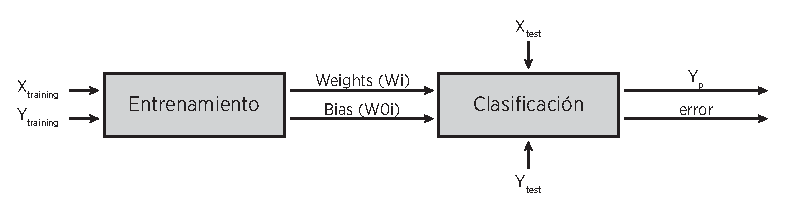
\includegraphics[width=\columnwidth]{imagenes/metodologia}
\caption{Metodologia}
\label{fig:metodologia}
\end{figure}

Se construyeron dos funciones en \emph{Matlab} para realizar el entrenamiento y la clasificación de los datos, así como una función adicional para mostrar el espacio particionado obtenido por el clasificador en cada uno de los ocho datasets proporcionados.

En Pseudocódigo \ref{alg:algoritmo-entrenamiento} se muestra el algoritmo general para realizar el entrenamiento con \emph{LDA}, el cual refleja los conceptos definidos en el marco teórico, específicamente en la Subsección \ref{sub:entrenamiento_del_lda}.

% function [Wi, W0i] = trainLDAmulti( Xtr, Ytr )
% dim = size(Xtr,1);

% gamma = unique(Ytr);
% c = max(gamma);
% Wi  = zeros(dim,c);
% W0i = zeros(dim,c);

% for i=1:c
%     % La clase c conocida sera el 1 en '1 vs todos'
%     c_instances = Xtr(:,Ytr==i);    % instancias de clase c
%     o_instances = Xtr(:,Ytr~=i);    % instancias de las otras clases
    
%     mu_1 = mean(c_instances,2);     % media de clase c
%     mu_2 = mean(o_instances,2);     % media del resto de las clases

%     S_1 = cov(c_instances');        % Matriz de covarianza de clase c
%     S_2 = cov(o_instances');        % Matriz de covarianza del resto de clases
       
%     Sw = S_1 + S_2;                 % Matriz de dispersión intra-clase Sw = S1 + S2
%     Wi(:,i) = Sw\(mu_1 - mu_2);     % Vector de pesos para clase c
%     W0i(:,i) = (mu_1 + mu_2)/2;     % Bias para clase c
% end
% end

\begin{algorithm} 
\footnotesize
\begin{algorithmic}[1] 
\REQUIRE  $Xtr$, $Ytr$
\ENSURE $Wi$ (matriz de vectores de proyección), $W0i$ (matriz de \emph{bias})
\FOR {Cada clase única $\omega_i$ en $Ytr$}
\STATE c\_inst = instancias de clase $\omega_i$ en $Xtr$
\STATE o\_inst = instancias no pertenecientes a clase $\omega_i$ en $Xtr$
\STATE $\mu_1$ = media de c\_inst
\STATE $\mu_2$ = media de o\_inst
\STATE $S_1$ = covarianza de c\_inst
\STATE $S_2$ = covarianza de o\_inst
\STATE $S_w$ = $S_1$ + $S_2$
\STATE $Wi$ = $S_w^{-1}*(\mu_1 - \mu_2)$
\STATE $W0i$ = $(\mu_1 + \mu_2)/2$
\ENDFOR
\end{algorithmic} 
\caption{Algoritmo de entrenamiento} 
\label{alg:algoritmo-entrenamiento}
\end{algorithm}

En Pseudocódigo \ref{alg:algoritmo-clasificacion} se muestra el algoritmo general para ejecutar la clasificación de los datos utilizando el enfoque \emph{uno vs todos}, utilizando los conceptos definidos en la Subsección \ref{sub:clasificacion}.

% function [ Yp, err ] = classifyLDAmulti( Xtt, Ytt, Wi, W0i )
% gamma = unique(Ytt);        % Clases en set de test
% c = max(gamma);             % Cantidad de clases distintas

% Pw_t = zeros(1,c);          % (auxiliar) Probabilidad de cada clase
% t_instances = size(Xtt,2);  % Total de instancias a clasificar

% Yp = zeros(1,t_instances);  % Etiquetas asignadas a cada instancia
% sigma_error = 0;            % Acumulador de errores

% for i=1:t_instances         % Por cada instancia ...
%     for j=1:c               % ... calcular su pertenencia a cada clase j
%         Pw_t(:,j) = Wi(:,j)' * ( Xtt(:,i) - W0i(:,j) ); 
%     end
%     [~,pred] = max(Pw_t);   % La clase asignada es la de mayor probabilidad
%     Yp(:,i) = pred;
%     sigma_error = sigma_error + (pred ~= Ytt(i)); % Incrementar error (si aplica)
% end

% err = (sigma_error * 100)/ t_instances; % Cálculo del porcentaje de error
% end

\begin{algorithm} 
\footnotesize
\begin{algorithmic}[1] 
\REQUIRE  $Xtt$, $Ytt$, $Wi$, $W0i$
\ENSURE $Yp$, $error$ (matriz de \emph{bias})
\FOR {Cada instancia $i$ en $Xtt$}
\FOR {Cada clase única $\omega_i$ en $Ytt$}
\STATE $P(\omega_i) = Wi' * ( x_i - W0i(:,j) )$
\ENDFOR
\STATE $Yp_i$ = max($P(\omega_i)$)
\ENDFOR
\end{algorithmic} 
\caption{Algoritmo de clasificación} 
\label{alg:algoritmo-clasificacion}
\end{algorithm}

Finalmente, en Pseudocódigo \ref{alg:algoritmo-visualizacion} se muestra el algoritmo utilizado para la creación de la gráfica con los espacios particionados, así como los puntos correcta e incorrectamente clasificados.


\begin{algorithm} 
\footnotesize
\begin{algorithmic}[1] 
\REQUIRE  $Xtt$,$Ytt$,$Ypred$,$Wi$,$W0i$
\ENSURE Una gráfica con el espacio particionado
\STATE $rango_x$ = crear 100 puntos entre min y max en X ($Xtt(1,:)$)
\STATE $rango_y$ = crear 100 puntos entre min y max en Y ($Xtt(2,:)$)
\STATE Crear una matriz $xy$ con los puntos sintéticos
\STATE Convertir matriz $xy$ a vector para clasificarlos con LDA, utilizando\\
$labels$ = classifyLDAmulti($xy$,$c$,$Wi$,$W0i$)
\STATE Transformar vector $labels$ a matriz (reshape)
\STATE Escalar y mostrar la matriz como el fondo (regiones particionadas) de la gráfica (imagesc)
\STATE Graficar puntos clasificados
\STATE Graficar los errores (puntos mal clasificados) según la diferencia entre $Ytt$ y $Ypred$
\end{algorithmic} 
\caption{Algoritmo de visualización} 
\label{alg:algoritmo-visualizacion}
\end{algorithm}


\section{Resultados} 
\label{sec:resultados}
La experimentación fue realizada en un equipo de cómputo con un procesador Intel core i7 de 8 núcleos a 2.00 GHz con 6 GB de memoria en RAM.
La Tabla \ref{tab:porcentajes-error} muestra los porcentajes de error obtenidos después de una iteración en cada uno de los 8 datasets proporcionados.

\begin{table}[h]
\centering
\caption{Porcentajes de error obtenidos por \emph{LDA}}
\label{tab:porcentajes-error}
\begin{tabular}{@{}cr@{}}
\toprule
\textbf{Dataset} & \multicolumn{1}{c}{\textbf{\% de Error}} \\ \midrule
clouds01         & 4.7222                                \\
clouds02         & 11.8                                  \\
clouds03         & 8.08                                  \\
clouds04         & 11.2782                               \\
clouds05         & 2.6667                                \\
clouds06         & 2.88                                  \\
clouds07         & 5.5                                   \\
clouds08         & 50                                    \\ \bottomrule
\end{tabular}

\end{table}

Las Figuras \cref{fig:lda-dataset-01,fig:lda-dataset-02,fig:lda-dataset-03,fig:lda-dataset-04,fig:lda-dataset-05,fig:lda-dataset-06,fig:lda-dataset-07,fig:lda-dataset-08} muestran el espacio particionado en cada uno de los datasets.
\begin{figure}[tb]
	\begin{center}
		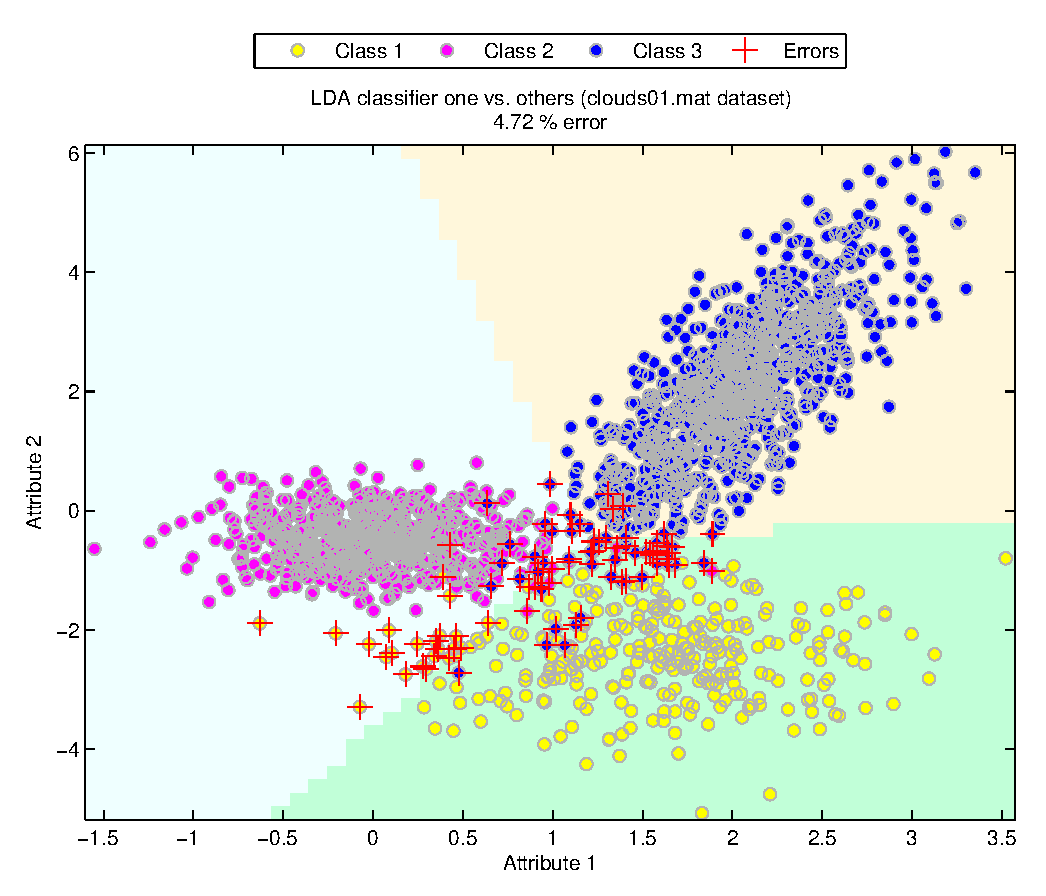
\includegraphics[width=\columnwidth]{imagenes/clouds01}
	\end{center}
	\caption{Espacio particionado en el dataset clouds01}
	\label{fig:lda-dataset-01}
\end{figure}

\begin{figure}[tb]
	\begin{center}
		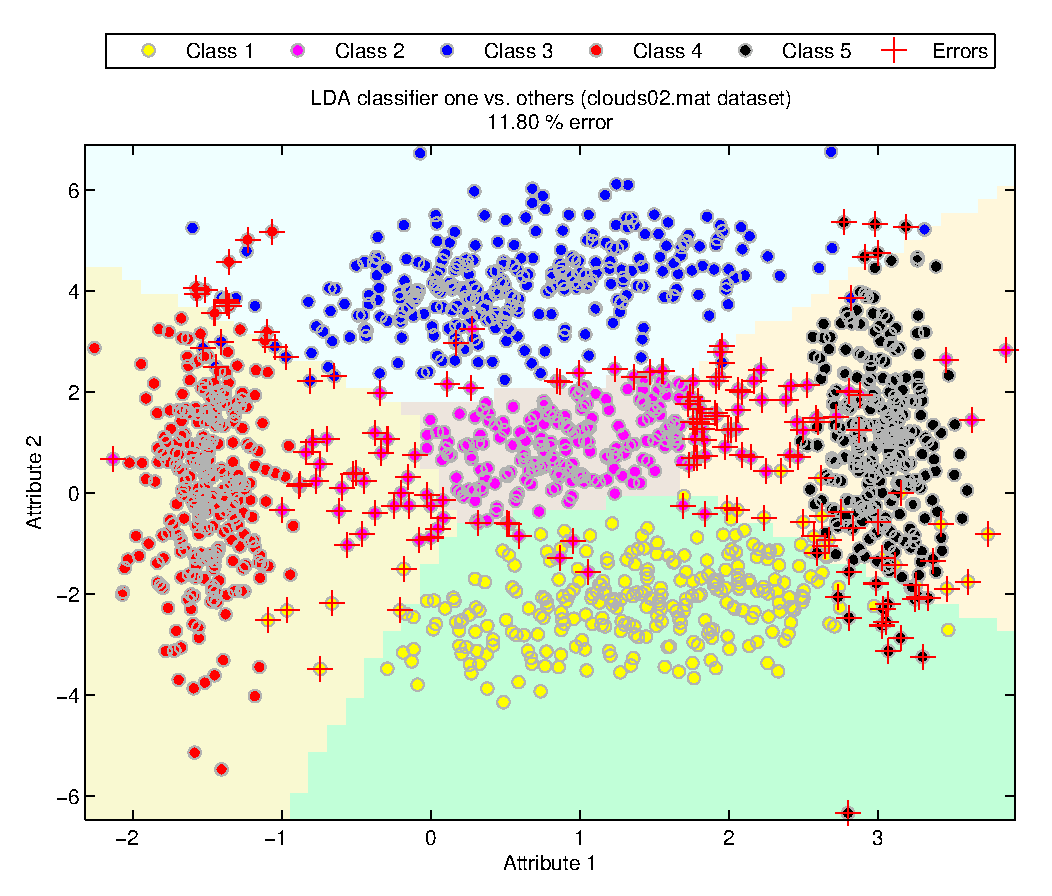
\includegraphics[width=\columnwidth]{imagenes/clouds02}
	\end{center}
	\caption{Espacio particionado en el dataset clouds02}
	\label{fig:lda-dataset-02}
\end{figure}

\begin{figure}[tb]
	\begin{center}
		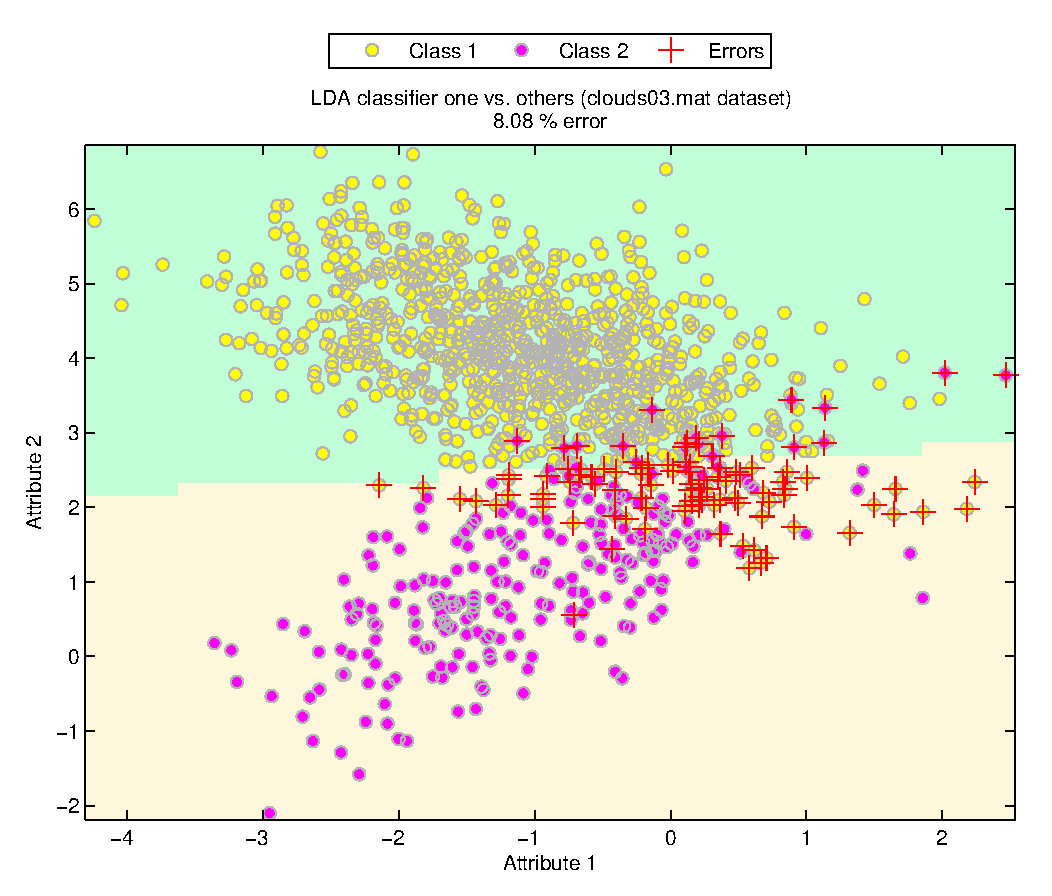
\includegraphics[width=\columnwidth]{imagenes/clouds03}
	\end{center}
	\caption{Espacio particionado en el dataset clouds03}
	\label{fig:lda-dataset-03}
\end{figure}

\begin{figure}[tb]
	\begin{center}
		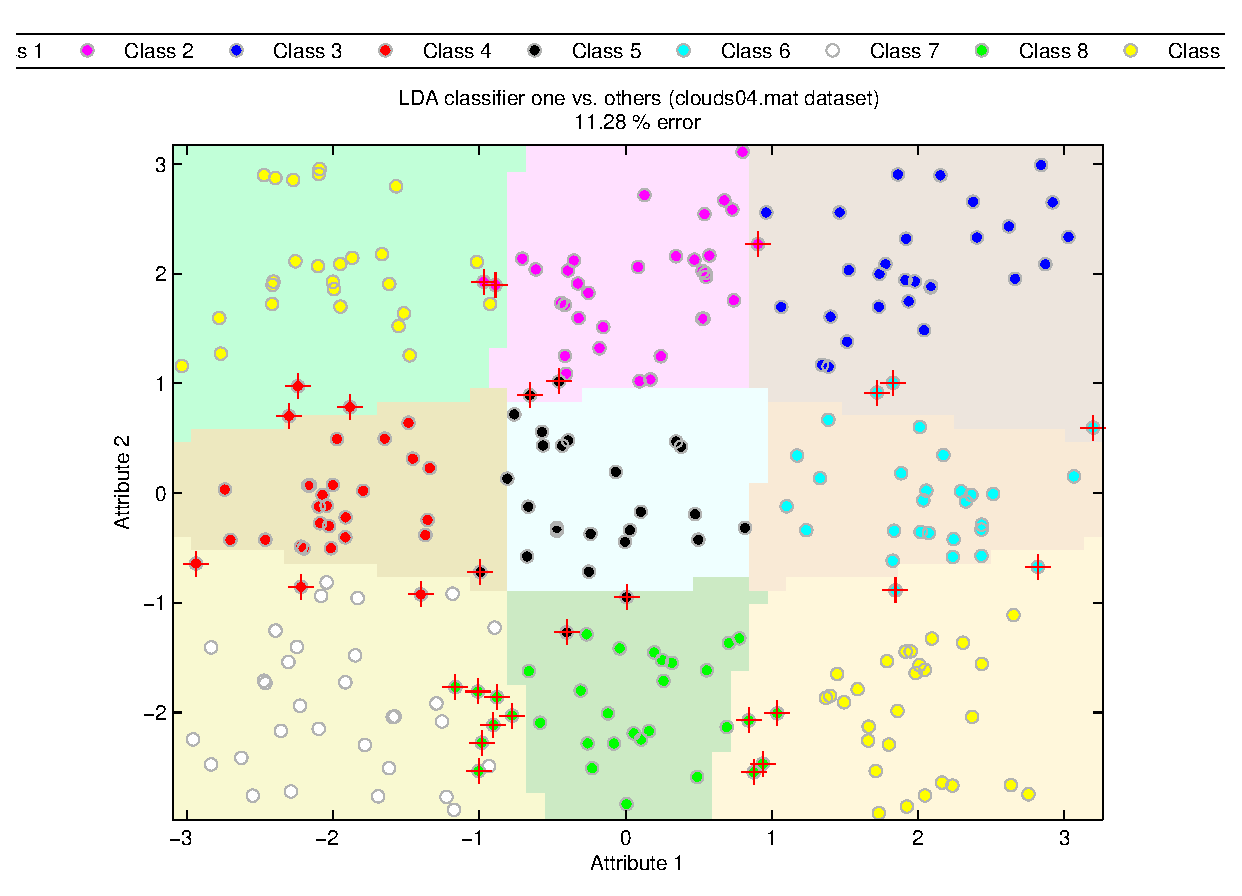
\includegraphics[width=\columnwidth]{imagenes/clouds04}
	\end{center}
	\caption{Espacio particionado en el dataset clouds04}
	\label{fig:lda-dataset-04}
\end{figure}

\begin{figure}[tb]
	\begin{center}
		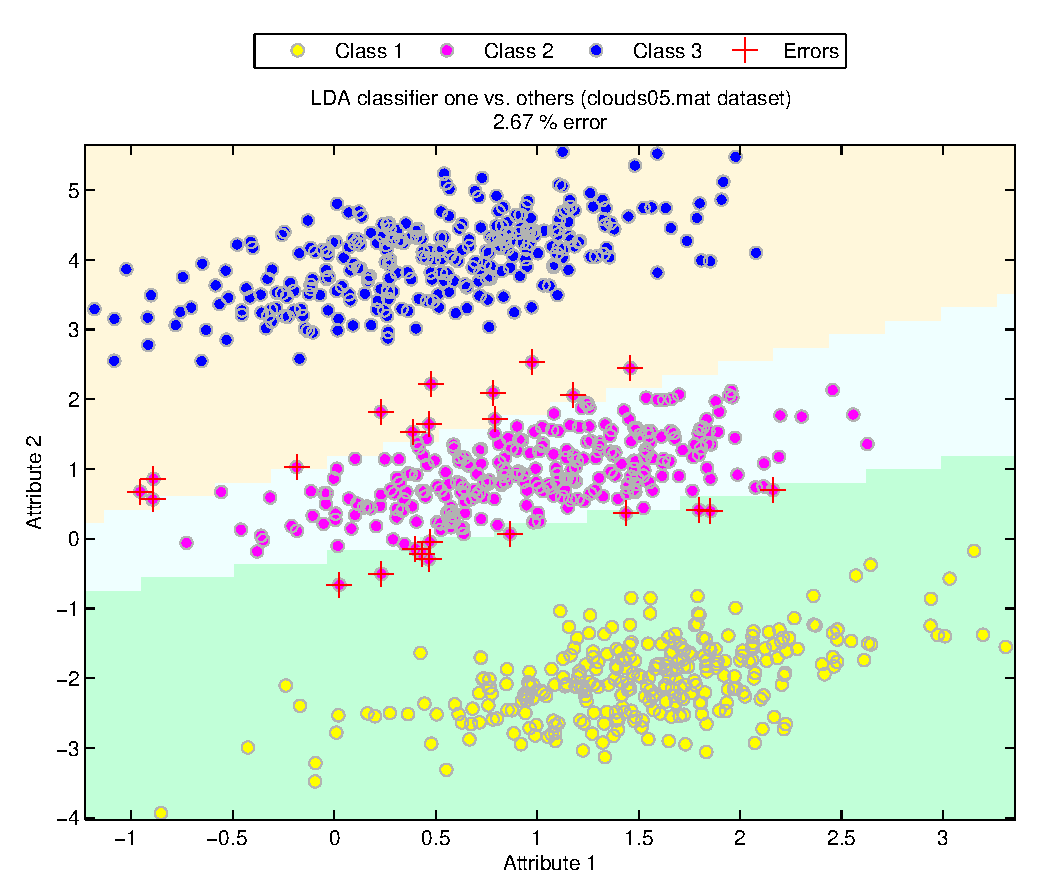
\includegraphics[width=\columnwidth]{imagenes/clouds05}
	\end{center}
	\caption{Espacio particionado en el dataset clouds05}
	\label{fig:lda-dataset-05}
\end{figure}

\begin{figure}[tb]
	\begin{center}
		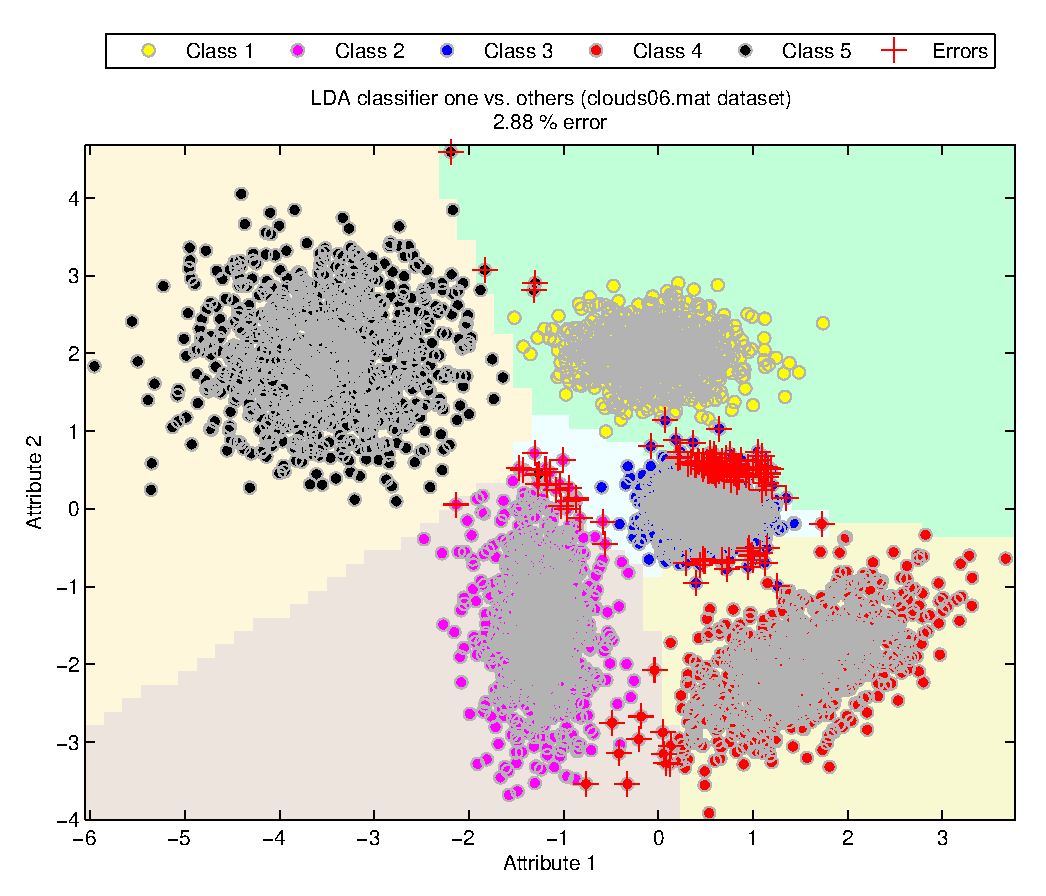
\includegraphics[width=\columnwidth]{imagenes/clouds06}
	\end{center}
	\caption{Espacio particionado en el dataset clouds06}
	\label{fig:lda-dataset-06}
\end{figure}

\begin{figure}[tb]
	\begin{center}
		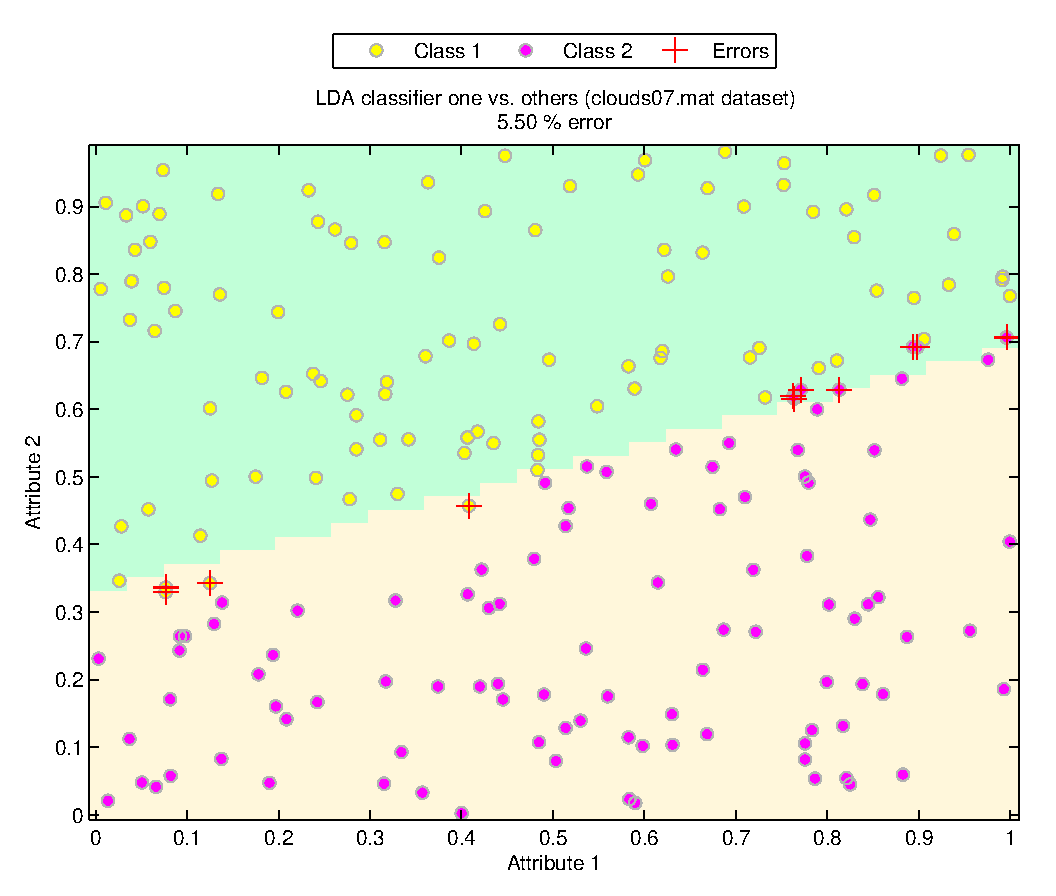
\includegraphics[width=\columnwidth]{imagenes/clouds07}
	\end{center}
	\caption{Espacio particionado en el dataset clouds07}
	\label{fig:lda-dataset-07}
\end{figure}

\begin{figure}[tb]
	\begin{center}
		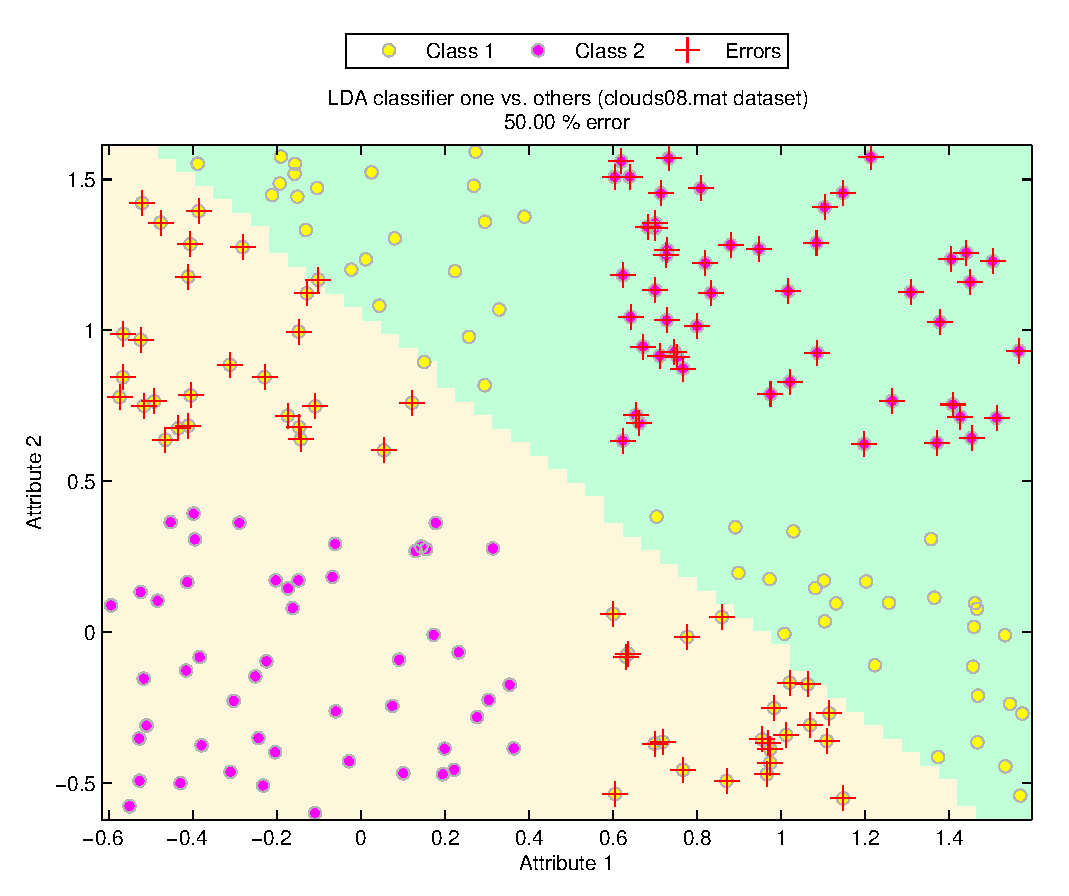
\includegraphics[width=\columnwidth]{imagenes/clouds08}
	\end{center}
	\caption{Espacio particionado en el dataset clouds08}
	\label{fig:lda-dataset-08}
\end{figure}

\section{Discusión de resultados}
\label{sec:discusion}
Como puede observarse en la tabla de resultados y en las figuras de las regiones particionadas para cada dataset, \emph{LDA} con el enfoque \emph{uno vs todos} obtiene \emph{buenos} resultados con porcentajes de error no mayores a 11.27\% (para los datasets proporcionados).
Sin embargo, hay una excepción a este comportamiento al considerar el último dataset (\ref{fig:lda-dataset-08})), para el cual se obtiene un 50\% de error en la clasificación.
Dicha situación puede ser originada debido a que las medias de las clases participantes están \emph{mezcladas} o a que los datos de dichas clases no sigan una distribución gaussiana, como es solicitado por \emph{LDA}.

Para el caso de datos linealmente separables, \emph{LDA} ofrece resultados rápidos con el beneficio de poder proyectarlos en un espacio de menor dimensionalidad.
Gracias a esto, si se requiere procesamiento adicional de los datos proyectados, ésto podría ser realizado necesitando menos poder de cómputo en comparación con los datos en su espacio de dimensiones original.

\section{Conclusiones}
\label{sec:conclusiones}
La técnica de \emph{LDA} permite reducir la dimensionalidad de los datos así como realizar labores de clasificación.
Para esta última tarea, y considerando que \emph{LDA} proporciona clasificación binaria, es preciso seguir un enfoque que permita realizar la clasificación multiclase como el \emph{uno vs todos} y el \emph{uno vs uno}.
Debido a que \emph{LDA} se basa en la idea de alcanzar una separabilidad utilizando la varianza y medias de los datos, ofrecerá buenos resultados si los datos a clasificar observan una distribución gaussiana.
En caso contrario, si los datos presentan valores de medias mezclados entre cada clase, los resultados no serán satisfactorios.

En este documento se ha presentado la descripción de una implementación de \emph{LDA} para realizar la clasificación multiclase utilizando un enfoque \emph{uno vs todos}, mostrando gráficas del espacio particionado por dicho clasificador y abordando además una pequeña discusión de sus resultados.

\nocite{*}
\bibliographystyle{ieeetran}
\bibliography{referencias}


\end{document}

